\section{Webová aplikace}

Frontendová část platformy, ve~formě webové aplikace a~aplikace mobilní je hlavní částí platformy, která živá data o~pohybu vozidel komunikuje k~cestujícím.

Využívá přitom komunikace s~Backendem za~pomocí REST + GraphQL API, vše za~využití protokolů HTTPS, nebo WebSocket.

Webová aplikace využívá technologie NextJS pro statické generování aplikace na~straně serveru (pro podporu SEO). Webová aplikace využívá za~svého chodu celou řadou doplňujících dotazů přes internet pro~dosažení interaktivity, takzvaných XHR requestů.

Vývojový model webové aplikace dopovídá programovacímu paradigma jednostránkové aplikace. \cite{singlepageapp}

\subsection{Mapa}
Na jednotné mapě se~zobrazují všechni dopravci. Mapu lze ovládat na~mobilních zařízeních pohyby prsty, nebo na~stolních počítačích myší. Podle uživatelského pohledu aplikace vybere dopravce, které by měla zobrazovat, čímž redukuje objem přenášených dat. Do~zařízení uživatele jsou přenášeny pouze data o~vozidlech, které uživatel sleduje.

Pro přehlednost mapa implementuje funkci shlukování vozidel do~bublin. Shlukování do~bublin zajistí v~aplikaci přehlednost a~plní i~funkci optimalizace výkonu mapy. Při vzdáleném pohledu je funkce plynulé animace pohybu vozidel vypnuta.
\begin{figure}[H]
    \centering
    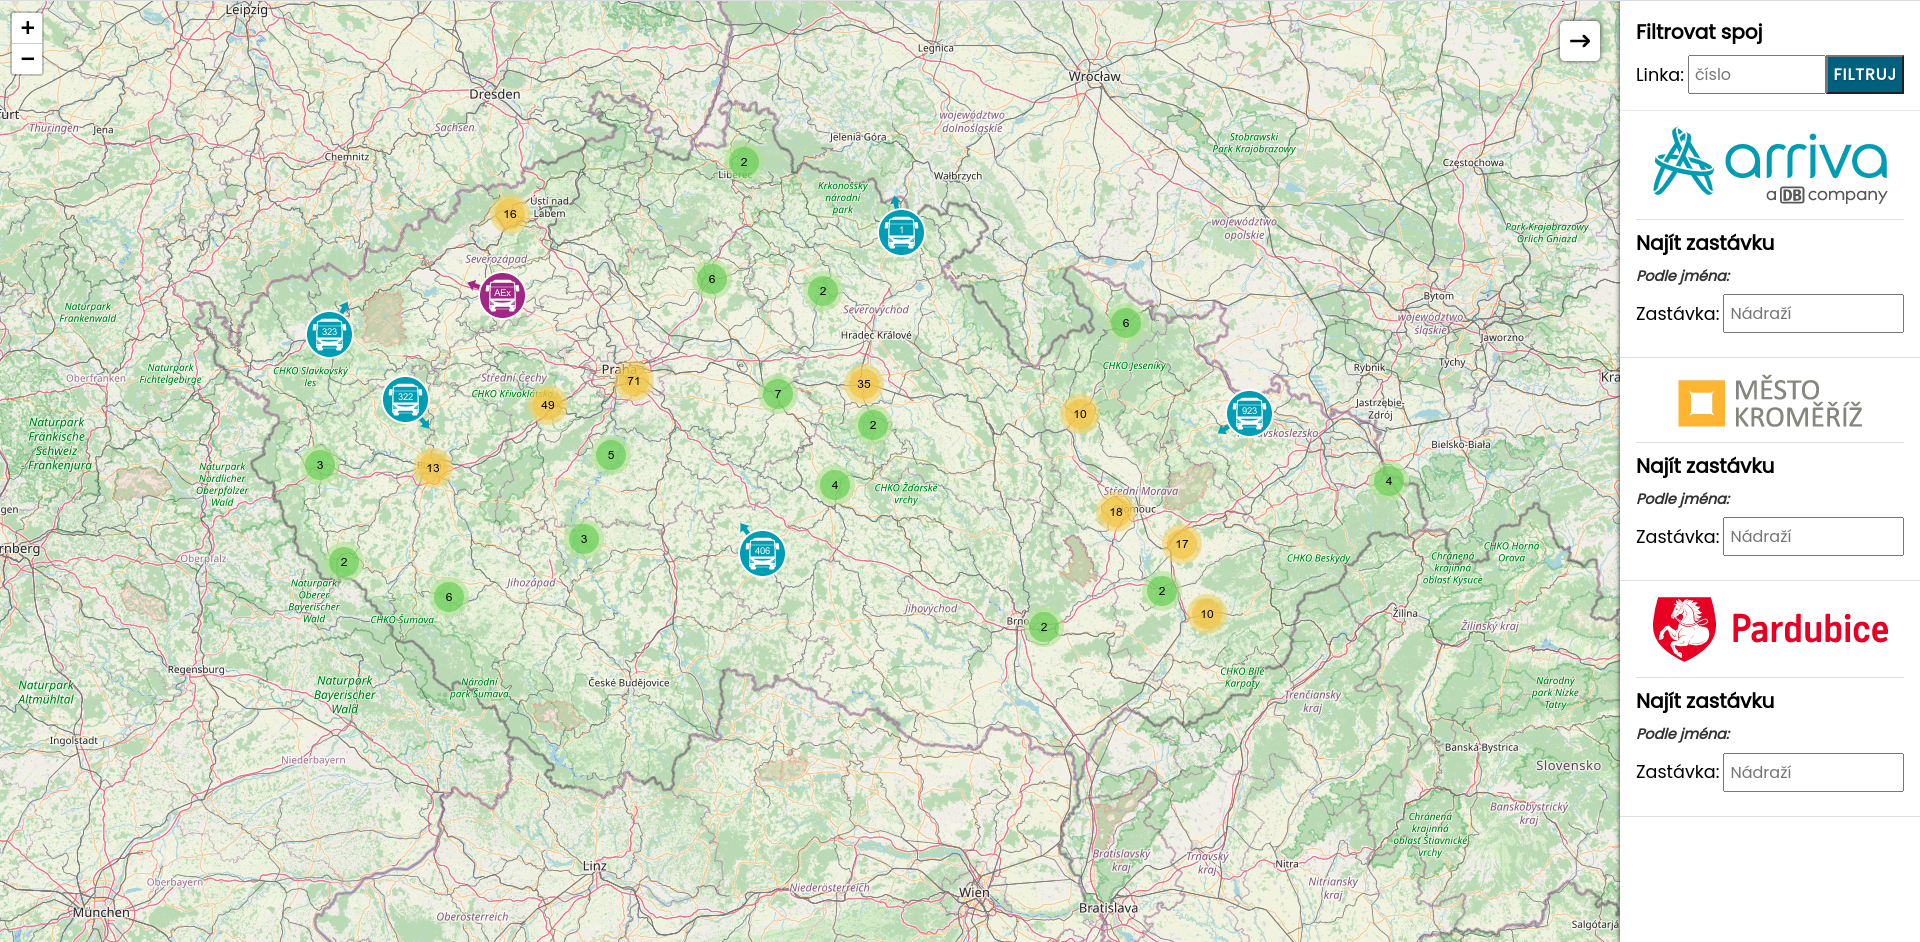
\includegraphics[width=1\textwidth]{images/global_map.png}
    \caption{Ukázka shlukování vozidel na~mapě}
    \label{shlukovani}
\end{figure}
\subsection{Zobrazování vozidel}
K~živému zobrazování dat se~využívá GraphQL subscription „GetVehicles“, díky které z~backendu automaticky přijde zpráva s~aktuálními daty. Tato data však mívají rozestup 10~sekund, proto se~animace plynulého přechodu dopočítává. Jednotlivá data vozidel jsou rozdělena podle dopravců, subscription se~tedy upravuje podle toho, kam se~uživatel zrovna dívá.
\begin{figure}[H]
    \centering
    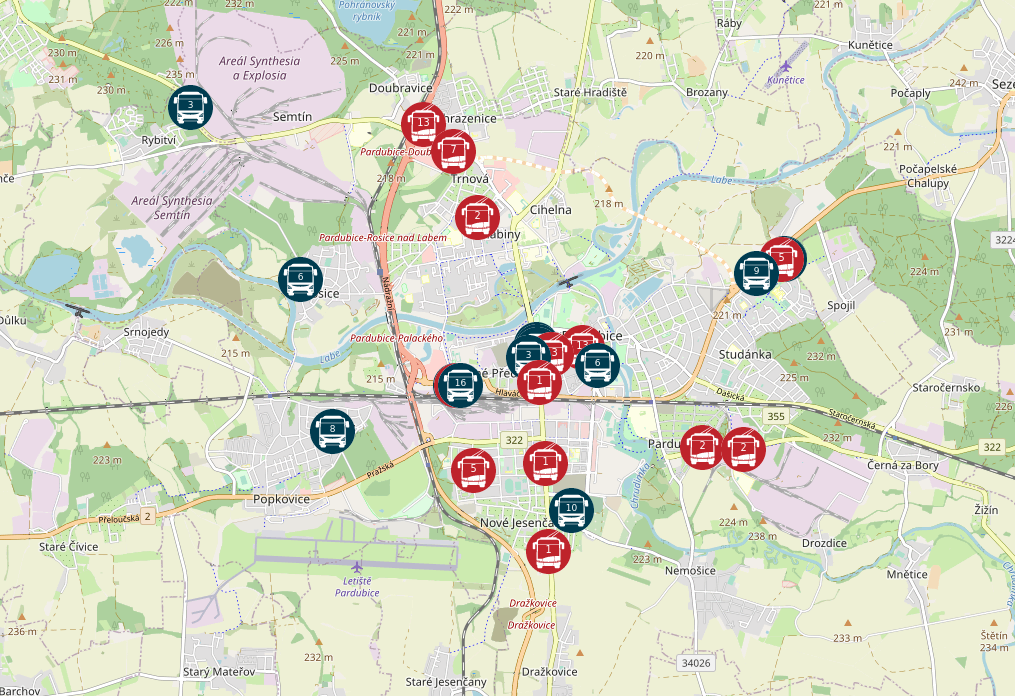
\includegraphics[width=1\textwidth]{images/Screenshot from 2023-03-18 20-15-00.png}
    \caption{Ukázka části mapy}
    \label{mapa}
\end{figure}

Pro dosažení plynulosti zobrazování využívá aplikace předepsaných praktik pro práci s~frameworkem ReactJS \ref{reactjs}. Časování animace přenechává aplikace webovému prohlížeči uživatele, využívá totiž Webového rozhraní Window.requestAnimationFrame() \cite{animationframe}, které zajišťuje vytváření nových snímků ve~vhodné frekvenci.
\subsection{Cache}
Informace o detailech spojení jsou na~straně cestujícího ukládána do~cache, aby již nebylo třeba tato data opakovaně načítat. Cache \ref{cache} na~straně webové aplikace šetří uživatelům jejich datové připojení a~zároveň snižují nároky na~vytěžování serveru.

\subsection{Detail spojení}
Uživatel má po~kliknutí na~jedoucí spoj k~dispozici základní informace o~tomto spoji, např. číslo linky, zpoždění, další zastávka, nebo cílová zastávka (viz obr.\ref{detail332}). Toto vše je vždy individálně upravitelné pro každý dopravní podnik. Po~rozkliknutí bližšího detailu o~spojení, se~uživateli zobrazí dodatečné informace (viz obr.\ref{detail7})

\begin{figure}[H]
    \centering
    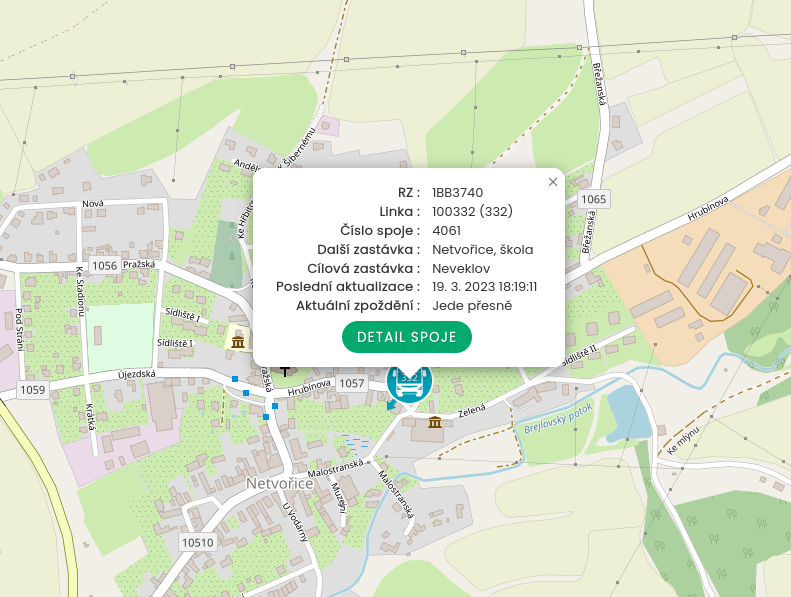
\includegraphics[width=0.6\textwidth]{images/small_detail.png}
    \caption{Detail linky 332}
    \label{detail332}
\end{figure}

\begin{figure}[H]
    \centering
    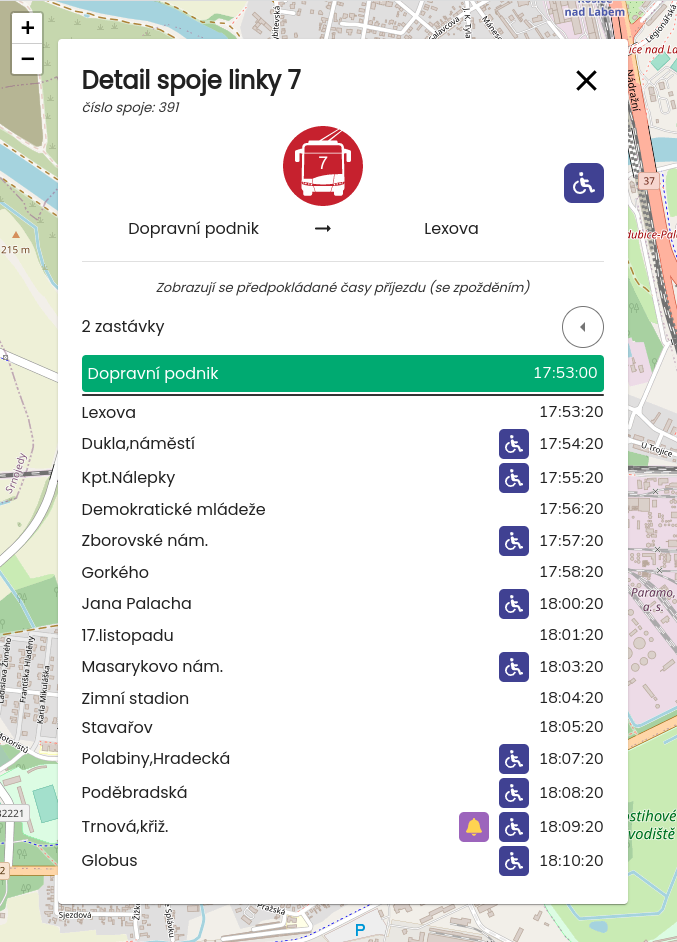
\includegraphics[width=0.6\textwidth]{images/global_pce_con_detail_7.png}
    \caption{Rozšířený detail linky 7}
    \label{detail7}
\end{figure}

Současně s~zobrazením bližších informací o~spoji se~zobrazuje také grafická reprezentace trasy, kudy daný spoj pojede, včetně zobrazení zastávek.

\begin{figure}[H]
    \centering
    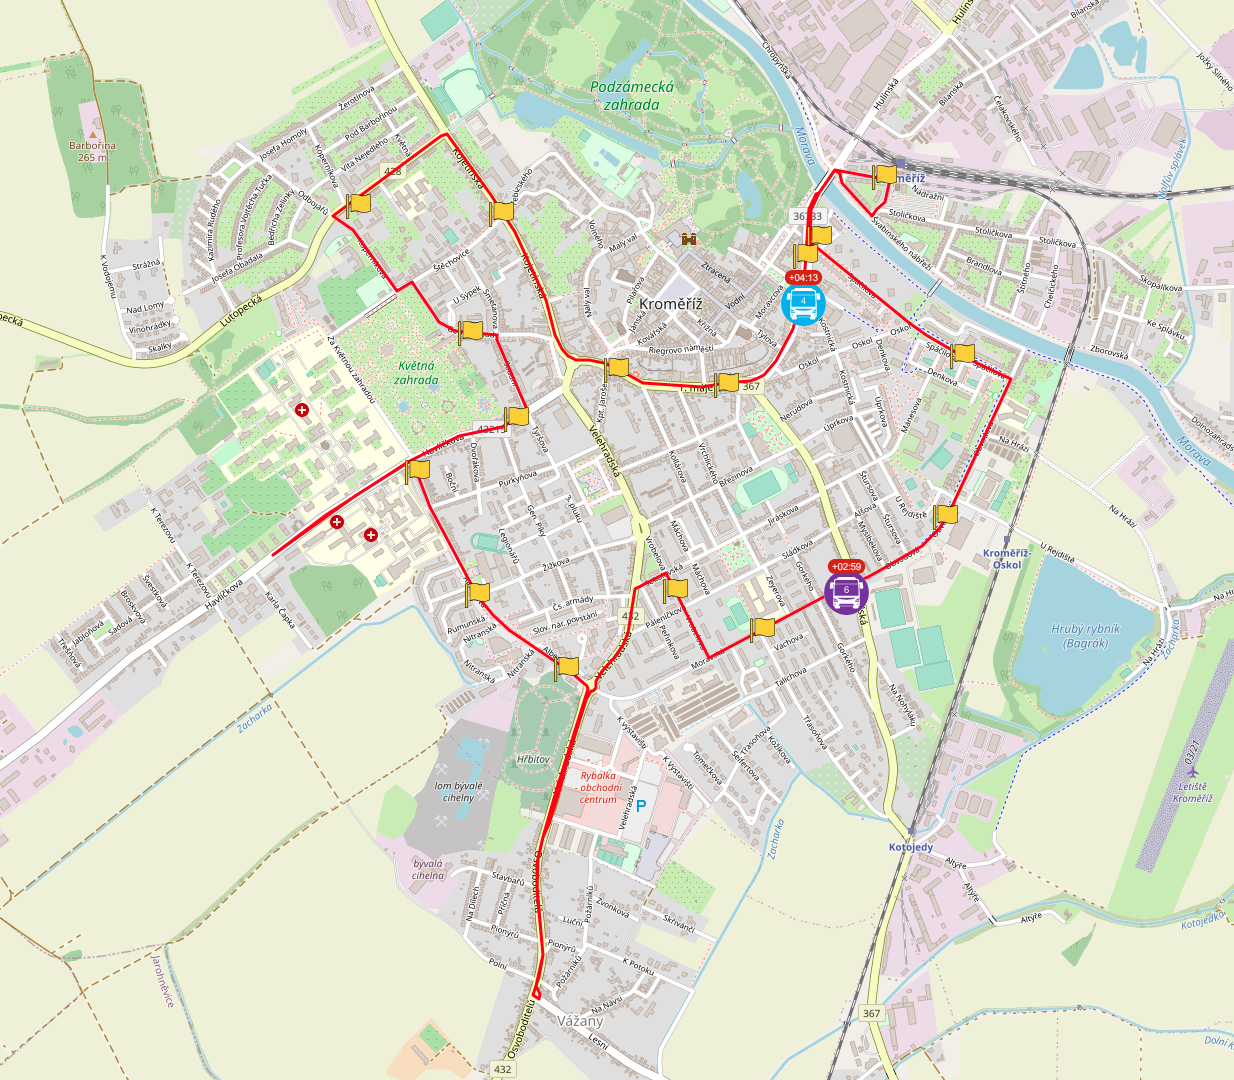
\includegraphics[width=0.7\textwidth]{images/krom_line_6.png}
    \caption{Detail trasy v~Kroměříži}
    \label{trasa}
\end{figure}

\subsection{Provozní upozornění} Dopravci mohou přidávat do~aplikace klienta provozní upozornění, které se~zobrazí v~případě, že se~vyskytne nějaká situace, která může mít vliv na~cestu cestujícího.\par
Za~tímto účelem vzniklo uživatelské prostředí pro dispečink dopravce.

Aplikace pravidelně zjistí aktuální stav a~zobrazí nejnovější informace.

\par \begin{figure}[H]
    \centering
    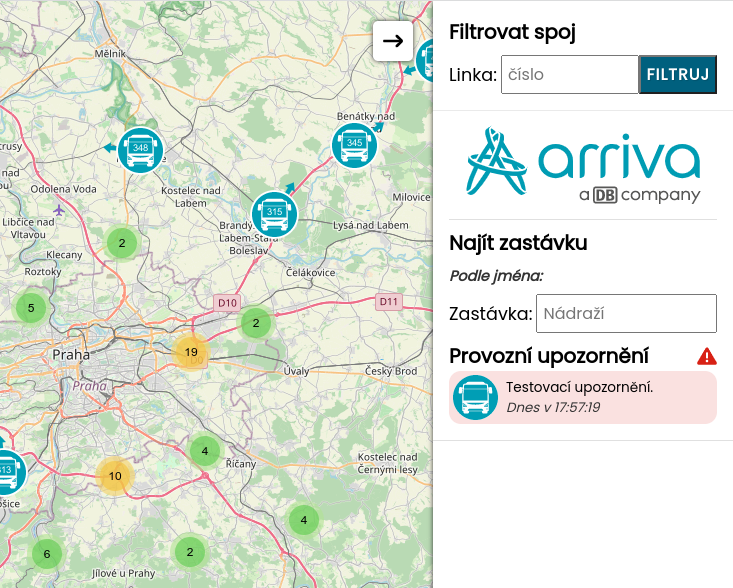
\includegraphics[width=0.75\textwidth]{images/global_arriva_event.png}
    \caption{Ukázka provozního upozornění}
    \label{upozorneni}
\end{figure}

\subsection{Práce s~polohou uživatele}
Aplikace na~požádání od~uživatele získá jeho aktuální polohu a~pro cestujícího v~zobrazí zastávky v~jeho blízkosti.

\begin{figure}[H]
    \centering
    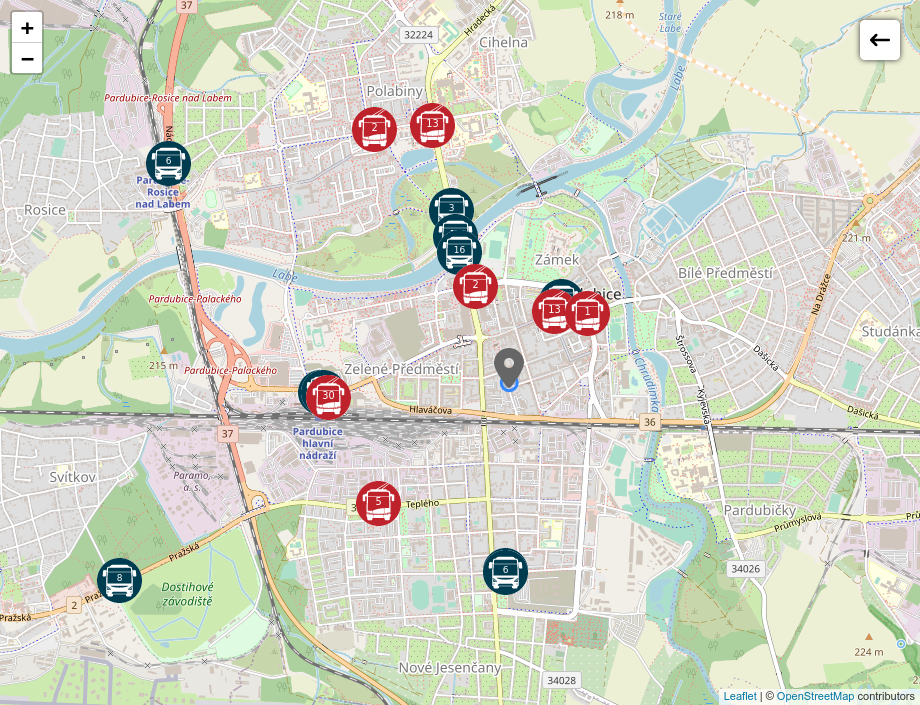
\includegraphics[width=0.75\textwidth]{images/position.png}
    \caption{Ukázka polohy uživatele}
    \label{poloha}
\end{figure}
\subsection{Monitorování návštěvnosti}
Zajímavou funkcí pro dopravce je monitorování návštěvnosti aplikace za~pomocí Google Analytics. Pro získávání přesných dat o~užitečných a~oblíbených funkcích aplikace využíváme monitorování vlastních událostí, např. při~otevření detailu spoje, nebo vyhledání detailu zastávky.
\subsection{Aplikace a~web}
Aplikace využívá experimentálních funkcí technologie PWA \ref{pwa} jako je například načítání GPS souřadnic uživatele, zobrazování notifikací, nastavení připomínky na~přijíždějící spoj. Funkce PWA zároveň nabízí stahování map do~zařízení, aby nemusely být při každém spuštění znovu stahovány.

Díky technologii PWA je webové aplikaci umožněno využít vnitřního uložiště zařízení pro ukládání dat o~mapách, a~tím je možné ušetřit uživatelům další stahování a~prodlevu před možností využívání aplikace.
